\documentclass{article}
\usepackage{graphicx}
\usepackage{amsmath, amssymb}
\usepackage{tikz}
\usetikzlibrary{calc, angles, quotes, arrows.meta, intersections}

\title{UR Computations in Geometric Optics Spring 2026}
\date{January 2026}

\begin{document}

\maketitle

\section{Week 1}

During the first week of research, we focused on defining the fundamental "lens-making problem" in geometric optics. The core of this problem is determining how to design the geometry of a lens so that light intensities from a source are redirected to specific points in 3D space. 

\subsection{Measuring Light Intensity}
We began by modeling light intensity in both 2D and 3D. In the 2D case, the source is represented by the unit circle $S^1$. If we consider a domain $\Omega \subseteq S^1$ and take an arc $A \subseteq \Omega$, the intensity of light passing through $A$ is given by the line integral:
\[ \int_A f(x) dx \]
where $f: \Omega \to \mathbb{R}$ is the density function and $x$ represents the position (often in radians). 

In 3D, the model shifts to the unit sphere $S^2$. To find the intensity through a specific patch $A \subseteq \Omega \subseteq S^2$, we use a surface integral:
\[ \int_A f(x) dx \]
In this context, $x$ is treated as a vector. We reviewed the necessary Calculus III concepts, specifically line and surface integrals, to handle these computations. We also discussed using polar and spherical coordinates to parameterize these regions.

\subsection{Lens Geometry and Reflection}
We defined the lens $R$ mathematically as the set of points:
\[ R = \{ \rho(x)x : x \in \Omega \} \]
where $\rho(x)$ represents the distance from the source to the lens surface.

Our initial technical goal is to study the uniform reflection properties of conics. Specifically, for a parabola defined by $y^2 = 4px$ (where $p$ is the focal length), we are working to prove the Law of Reflection: that the angle of incidence equals the angle of reflection. This proof involves a step-by-step geometric approach:
\begin{enumerate}
    \item Finding the equation of the normal line $N$ and the slope of the tangent at a point $P$.
    \item Calculating the slope of the segment $\overline{FP}$, where $F$ is the focus $(p, 0)$.
    \item Determining the slope of the reflected line $\ell$.
    \item Using these slopes to verify that the angle between $\ell$ and $N$ is equal to the angle between $\overline{FP}$ and $N$.
\end{enumerate}
This framework will eventually be extended to study the refraction properties of ellipses.

\subsection{Geometric Setup}
We consider a parabola defined by the equation $y^2 = 4px$, where $p$ is the focal length. The focus $F$ is located at $(p, 0)$. Let $P(x, y)$ be an arbitrary point on the parabola. 

\begin{figure}[h]
    \centering
    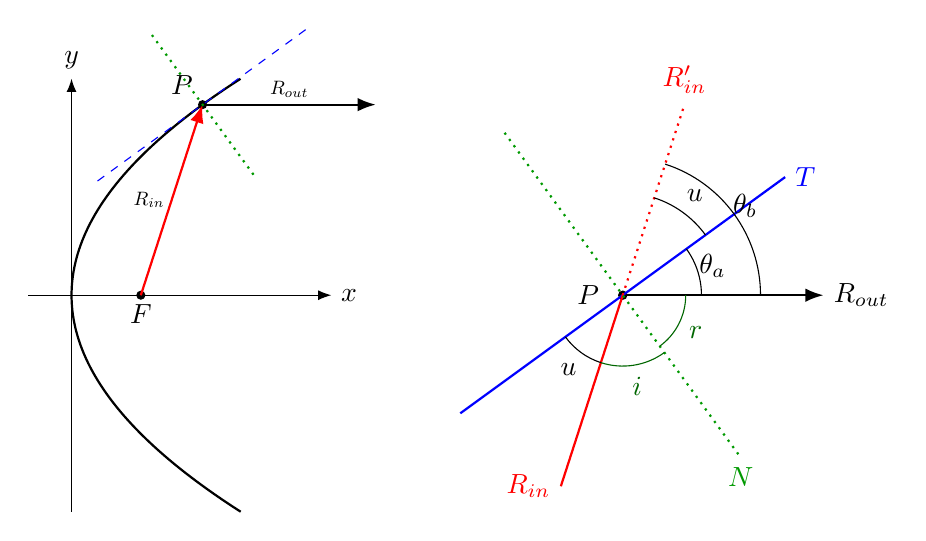
\begin{tikzpicture}[>=Latex]
        
        % --- PARAMETERS ---
        \def\p{0.8}
        \def\yP{2.2}
        \pgfmathsetmacro{\xP}{\yP*\yP/(4*\p)}
        
        % ANGLES
        % Tangent Angle: tan(theta) = 2p/y
        \pgfmathsetmacro{\angTan}{atan(2*\p/\yP)}
        % Incident Angle: Slope from Focus to P
        \pgfmathsetmacro{\angIncGeo}{atan(\yP/(\xP-\p))}
        % Normal Angle: Tangent - 90 (pointing down-right)
        \pgfmathsetmacro{\angNorm}{\angTan - 90}
        
        % --- MAIN DIAGRAM (LEFT) ---
        \begin{scope}[scale=1.1]
            \draw[->] (-0.5,0) -- (3,0) node[right] {$x$};
            \draw[->] (0,-2.5) -- (0,2.5) node[above] {$y$};
            \draw[thick, domain=-2.5:2.5, samples=100, variable=\t] plot ({\t*\t/(4*\p)}, \t);
            \coordinate (F) at (\p, 0);
            \coordinate (P) at (\xP, \yP);
            \fill (F) circle (1.5pt) node[below] {$F$};
            \fill (P) circle (1.5pt) node[above left] {$P$};
            
            % Rays
            \draw[red, thick, ->] (F) -- (P) node[midway, left, scale=0.7, text=black] {$R_{in}$};
            % R_out changed to BLACK
            \draw[black, thick, ->] (P) -- ++(2.0, 0) coordinate (Refl) node[midway, above, scale=0.7, text=black] {$R_{out}$};
            
            % Tangent
            \draw[blue, dashed] ($(P) + ({180+\angTan}:1.5)$) -- ($(P) + ({\angTan}:1.5)$);
            
            % Normal (Made thicker/bolder)
            \draw[green!60!black, thick, dotted] ($(P) + ({\angNorm}:1.0)$) -- ($(P) + ({\angNorm+180}:1.0)$);
        \end{scope}

        % --- ZOOM DIAGRAM (RIGHT) ---
        \begin{scope}[shift={(7,0)}, scale=1.7]
            \coordinate (C) at (0,0);
            \node[left, xshift=-5pt] at (C) {$P$};
            \fill (C) circle (1pt);
            
            % COORDINATES
            \coordinate (Right) at (1.5,0); % Horizontal Right (Reflected)
            \coordinate (T_top) at ({\angTan}:1.5); % Tangent Top-Right
            \coordinate (T_bot) at ({180+\angTan}:1.5); % Tangent Bottom-Left
            \coordinate (R_in_src) at ({180+\angIncGeo}:1.5); % Incident Source (Bottom-Left)
            \coordinate (R_in_ext) at ({\angIncGeo}:1.5); % Incident Extended (Top-Right)
            \coordinate (N_bot) at ({\angNorm}:1.5); % Normal (Bottom-Right)
            \coordinate (N_top) at ({\angNorm+180}:1.5); % Normal (Top-Left)
            
            % LINES
            % 1. Horizontal Reflected
            \draw[thick, ->] (C) -- (Right) node[right] {$R_{out}$};
            
            % 2. Tangent (Solid Blue)
            \draw[blue, thick] (T_bot) -- (T_top) node[right] {$T$};
            
            % 3. Incident Ray (Red)
            \draw[red, thick] (R_in_src) node[left] {$R_{in}$} -- (C);
            \draw[red, thick, dotted] (C) -- (R_in_ext) node[above] {$R'_{in}$};
            
            % 4. Normal (Green Dotted, Extended)
            \draw[green!60!black, thick, dotted] (N_top) -- (N_bot) node[below] {$N$};
            
            % --- ANGLES ---
            
            % 1. Theta_a: Horizontal to Tangent (Right Side)
            \pic [draw, "$\theta_a$", angle radius=1.0cm, angle eccentricity=1.2] {angle = Right--C--T_top};
            
            % 2. Theta_b: Horizontal to Extended Incident (Right Side)
            % SCALED DOWN radius to 1.75cm
            \pic [draw, "$\theta_b$", angle radius=1.75cm, angle eccentricity=1.1] {angle = Right--C--R_in_ext};
            
            % 3. u (Right Side): Tangent to Extended Incident
            \pic [draw, "$u$", angle radius=1.3cm, angle eccentricity=1.2] {angle = T_top--C--R_in_ext};
            
            % 4. u (Left Side): Tangent to Incident
            \pic [draw, "$u$", angle radius=0.9cm, angle eccentricity=1.3] {angle = T_bot--C--R_in_src};
            
            % 5. Reflection Angle r: Normal to Horizontal
            \pic [draw, "$r$", angle radius=0.8cm, angle eccentricity=1.3, color=green!40!black] {angle = N_bot--C--Right};
            
            % 6. Incidence Angle i: Incident Source to Normal
            \pic [draw, "$i$", angle radius=0.9cm, angle eccentricity=1.3, color=green!40!black] {angle = R_in_src--C--N_bot};

        \end{scope}
    \end{tikzpicture}
    \caption{Reflection in a Parabola. The geometric proof relies on the relationship $\theta_a = 2\theta_b$, visually verified by the extended incident ray and the tangent.}
    \label{fig:parabola_reflection}
\end{figure}

The Law of Reflection requires the angle of incidence ($\alpha_i$) to equal the angle of reflection ($\alpha_r$) relative to the normal line $N$. To show that the condition $\theta_a = 2\theta_b$ satisfies this law for a horizontal reflected ray, we observe the following geometry:

\begin{itemize}
    \item The normal line $N$ is perpendicular to the tangent, so its angle relative to the horizontal is $90^\circ + \theta_b$.
    \item A horizontal reflected ray makes an angle of $\theta_b$ with the tangent line. Therefore, the angle of reflection relative to the normal is $\alpha_r = 90^\circ - \theta_b$.
    \item By the Law of Reflection, the angle of incidence must also be $\alpha_i = 90^\circ - \theta_b$.
\end{itemize}

We calculate the incident ray angle $\theta_a$ by subtracting the angle of incidence from the angle of the normal:
\[ \theta_a = (90^\circ + \theta_b) - (90^\circ - \theta_b) = 2\theta_b \]

This confirms that proving $\tan(\theta_a) = \tan(2\theta_b)$ is geometrically equivalent to satisfying the Law of Reflection for rays reflecting parallel to the $x$-axis.

\subsection{Proof using the Double-Angle Identity}
First, we find the slope of the tangent line at $P(x, y)$ by differentiating the parabola's equation with respect to $x$:
\[ 2y \frac{dy}{dx} = 4p \implies \frac{dy}{dx} = \frac{2p}{y} \]
Substituting $y = \sqrt{4px}$, we obtain the tangent slope, which we define as $\tan(\theta_b)$:
\[ \tan(\theta_b) = \frac{2p}{\sqrt{4px}} = \frac{2p}{2\sqrt{px}} = \sqrt{\frac{p}{x}} \]

Next, we calculate the slope of the incident ray from the focus $F(p, 0)$ to the point $P(x, y)$. This slope represents $\tan(\theta_a)$:
\[ \tan(\theta_a) = \frac{y - 0}{x - p} = \frac{\sqrt{4px}}{x - p} \]

Finally, we apply the tangent double-angle identity, $\tan(2\theta) = \frac{2\tan\theta}{1 - \tan^2\theta}$, to $\theta_b$:
\[ \tan(2\theta_b) = \frac{2\sqrt{\frac{p}{x}}}{1 - \left(\sqrt{\frac{p}{x}}\right)^2} = \frac{2\sqrt{\frac{p}{x}}}{1 - \frac{p}{x}} \]
Multiplying the numerator and denominator by $x$:
\[ \tan(2\theta_b) = \frac{2x\sqrt{\frac{p}{x}}}{x - p} = \frac{2\sqrt{px}}{x - p} = \frac{\sqrt{4px}}{x - p} \]

Since $\tan(2\theta_b) = \frac{\sqrt{4px}}{x - p} = \tan(\theta_a)$, we have proven that $\theta_a = 2\theta_b$. This confirms that the reflected ray is perfectly horizontal, verifying the uniform reflection property of the parabola.

\section{Week 2: Uniform Refraction Property of the Ellipse}

This week, we prove the fundamental "lens-making" property of an elliptical boundary. Specifically, we show that rays originating from a focus $F_1$ and passing into a second medium will emerge parallel to the major axis if the ratio of the refractive indices is equal to the eccentricity of the ellipse.

\subsection{Geometric Setup and the Rotation Trick}
Consider an ellipse defined by $\frac{x^2}{a^2} + \frac{y^2}{b^2} = 1$, with $a^2 = b^2 + c^2$. Let the source be at the focus $F_1(-c, 0)$. 

\begin{figure}[h]
    \centering
    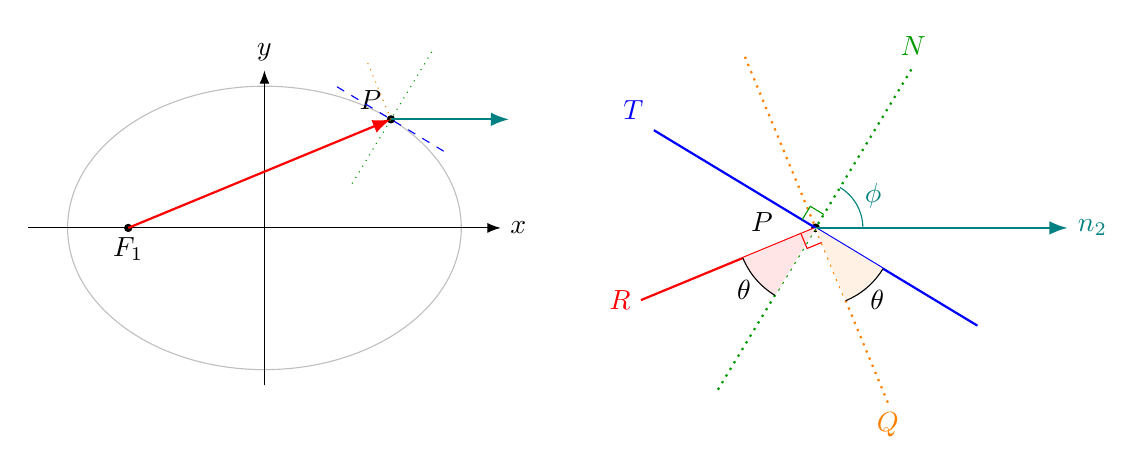
\begin{tikzpicture}[>=Latex]
        
        % --- PARAMETERS ---
        \def\a{2.5} \def\b{1.8} \def\c{1.73}
        \def\angParam{50} 
        \pgfmathsetmacro{\angRay}{atan2(\b*sin(\angParam), \a*cos(\angParam) + \c)}
        \pgfmathsetmacro{\angTan}{atan2(\b*cos(\angParam), -\a*sin(\angParam))}
        \pgfmathsetmacro{\angNorm}{\angTan - 90}
        \pgfmathsetmacro{\angAux}{\angRay - 90}

        % --- MAIN DIAGRAM (LEFT) ---
        \begin{scope}[scale=1.0]
            \draw[gray!50] (0,0) ellipse ({\a} and {\b});
            \draw[->] (-3,0) -- (3,0) node[right] {$x$};
            \draw[->] (0,-2) -- (0,2) node[above] {$y$};
            \coordinate (F1) at (-\c, 0);
            \coordinate (P) at ({\a*cos(\angParam)}, {\b*sin(\angParam)});
            \fill (F1) circle (1.5pt) node[below] {$F_1$};
            \fill (P) circle (1.5pt) node[above left] {$P$};
            \draw[red, thick, ->] (F1) -- (P);
            \draw[teal, thick, ->] (P) -- ++(1.5, 0); 
            \draw[blue, dashed] ($(P) + ({\angTan}:0.8)$) -- ($(P) + ({\angTan+180}:0.8)$);
            \draw[green!60!black, dotted] ($(P) + ({\angNorm}:1.0)$) -- ($(P) + ({\angNorm-180}:1.0)$);
            \draw[orange, dotted] (P) -- ($(P)!0.8cm!-90:(F1)$); 
        \end{scope}

        % --- ZOOM DIAGRAM (RIGHT) ---
        \begin{scope}[shift={(7,0)}, scale=1.6]
            \coordinate (C) at (0,0);
            \node[left, xshift=-12pt, yshift=2pt] at (C) {$P$}; 
            \fill (C) circle (1pt);
            
            % Vectors
            \coordinate (R_in) at ({\angRay+180}:1.5); 
            \coordinate (R_line) at ({\angRay}:1.5);
            \coordinate (Q_top) at ({\angAux+180}:1.5);
            \coordinate (Q_bot) at ({\angAux}:1.5);
            \coordinate (N_top) at ({\angNorm}:1.5);
            \coordinate (N_bot) at ({\angNorm-180}:1.5); 
            \coordinate (T_top) at ({\angTan}:1.5);
            \coordinate (T_bot) at ({\angTan-180}:1.5);
            \coordinate (Refracted) at (2.0,0);
            
            % --- LINES ---
            \draw[red, thick] (R_in) node[left] {$R$} -- (C);
            \draw[orange, thick, dotted] (Q_bot) node[below] {$Q$} -- (Q_top);
            \draw[green!60!black, thick, dotted] (N_bot) -- (N_top) node[above] {$N$};
            \draw[blue, thick] (T_bot) -- (T_top) node[above left] {$T$};
            \draw[teal, thick, ->] (C) -- (Refracted) node[right] {$n_2$};
            
            % --- ANGLES ---
            \pic [draw, "$\theta$", angle radius=1.0cm, angle eccentricity=1.2, fill=red!10] {angle = R_in--C--N_bot};
            \pic [draw, "$\theta$", angle radius=1.0cm, angle eccentricity=1.2, fill=orange!10] {angle = Q_bot--C--T_bot};
            \pic [draw, "$\phi$", angle radius=0.6cm, angle eccentricity=1.4, teal] {angle = Refracted--C--N_top};
            
            % Right Angle Markers
            \pic [draw, angle radius=0.2cm, color=red] {right angle = R_in--C--Q_bot};
            \pic [draw, angle radius=0.2cm, color=green!60!black] {right angle = N_top--C--T_top};

        \end{scope}
    \end{tikzpicture}
    \caption{Refraction in an Ellipse. The "Rotation Trick": Since $Q \perp R$ and $T \perp N$, the angle $\theta$ between $Q$ and $T$ must equal the angle of incidence (between $R$ and $N$).}
    \label{fig:ellipse_refraction}
\end{figure}

\begin{itemize}
    \item \textbf{Incident Ray ($R$):} A ray travels from $F_1$ to an arbitrary point $P(x, y)$ on the ellipse. Its slope is $m_R = \frac{y}{x+c}$.
    \item \textbf{Tangent Line ($T$):} By implicit differentiation, the slope of the tangent at $P$ is $m_T = -\frac{b^2x}{a^2y}$.
    \item \textbf{The Auxiliary Line ($Q$):} To simplify the calculation of the angle of incidence $\theta$ (the angle between $R$ and the normal $N$), we define a line $Q$ perpendicular to $R$ at point $P$. Its slope is the negative reciprocal of $m_R$:
    \[ m_Q = -\frac{1}{m_R} = -\frac{x+c}{y} \]
    Because $N \perp T$ and $R \perp Q$, the angle between $N$ and $R$ is identical to the angle between $T$ and $Q$. Thus, $\theta$ is the angle between the tangent and our auxiliary line $Q$.
\end{itemize}

\subsection{Calculating the Angle of Incidence $\theta$}
We use the tangent subtraction formula to find $\tan \theta$:
\begin{equation}
    \tan \theta = \frac{m_T - m_Q}{1 + m_T m_Q} = \frac{-\frac{b^2x}{a^2y} - \left(-\frac{x+c}{y}\right)}{1 + \left(-\frac{b^2x}{a^2y}\right)\left(-\frac{x+c}{y}\right)} = \frac{\frac{x+c}{y} - \frac{b^2x}{a^2y}}{1 + \frac{b^2(x^2+cx)}{a^2y^2}}
\end{equation}
To simplify, multiply the numerator and denominator by $a^2y^2$:
\begin{equation}
    \tan \theta = \frac{a^2y(x+c) - b^2xy}{a^2y^2 + b^2x^2 + b^2cx}
\end{equation}
Applying the ellipse identity $a^2y^2 + b^2x^2 = a^2b^2$ in the denominator and expanding the numerator:
\begin{equation}
    \tan \theta = \frac{a^2xy + a^2cy - b^2xy}{a^2b^2 + b^2cx} = \frac{(a^2-b^2)xy + a^2cy}{b^2(a^2 + cx)} = \frac{c^2xy + a^2cy}{b^2(a^2+cx)} = \frac{cy(cx+a^2)}{b^2(a^2+cx)} = \frac{cy}{b^2}
\end{equation}

\subsection{Calculating the Angle of Refraction $\phi$}
Let $\phi$ be the angle of refraction. Since we require the refracted ray to be parallel to the major axis (horizontal), $\phi$ is simply the angle between the normal line $N$ and the horizontal. The slope of the normal is $m_N = \frac{a^2y}{b^2x}$, so:
\begin{equation}
    \tan \phi = m_N = \frac{a^2y}{b^2x}
\end{equation}

\subsection{Verification via Snell's Law}
To apply Snell's Law $n_1 \sin \theta = n_2 \sin \phi$, we convert the tangents to sines using $\sin \alpha = \frac{\tan \alpha}{\sqrt{1+\tan^2 \alpha}}$.
\begin{itemize}
    \item \textbf{For incidence:} $\sin \theta = \frac{cy/b^2}{\sqrt{1 + (cy/b^2)^2}} = \frac{cy}{\sqrt{b^4 + c^2y^2}}$
    \item \textbf{For refraction:} $\sin \phi = \frac{a^2y/b^2x}{\sqrt{1 + (a^2y/b^2x)^2}} = \frac{a^2y}{\sqrt{b^4x^2 + a^4y^2}}$
\end{itemize}
We simplify the radical in $\sin \phi$ using the substitution $b^2x^2 = a^2b^2 - a^2y^2$:
\begin{equation}
    \sqrt{b^4x^2 + a^4y^2} = \sqrt{b^2(a^2b^2 - a^2y^2) + a^4y^2} = \sqrt{a^2b^4 - a^2b^2y^2 + a^4y^2} = \sqrt{a^2b^4 + a^2y^2(a^2-b^2)}
\end{equation}
Since $a^2 - b^2 = c^2$, this simplifies to $a\sqrt{b^4 + c^2y^2}$. Substituting this back:
\begin{equation}
    \sin \phi = \frac{a^2y}{a\sqrt{b^4 + c^2y^2}} = \frac{ay}{\sqrt{b^4 + c^2y^2}}
\end{equation}

\subsection{Conclusion}
Taking the ratio of the sines:
\begin{equation}
    \frac{\sin \phi}{\sin \theta} = \frac{ay}{cy} = \frac{a}{c}
\end{equation}
From Snell's Law, $n_1 \sin \theta = n_2 \sin \phi \implies \frac{n_1}{n_2} = \frac{\sin \phi}{\sin \theta}$. Therefore:
\begin{equation}
    \frac{n_1}{n_2} = \frac{a}{c} \implies \frac{n_2}{n_1} = \frac{c}{a} = e
\end{equation}
This proves that if the refractive index of the outer medium relates to the inner medium by the eccentricity of the ellipse ($n_2 = n_1 \cdot e$), all rays from the focus emerge parallel to the major axis. 

\section{Week 3: Computational Simulations and Vector Formulations}

During the third week, we transitioned from scalar geometric proofs to computational modeling and vector-based physics. This allowed for the visualization of "fans" of rays and the derivation of formulas suitable for computer graphics and ray-tracing algorithms.

\subsection{Program Descriptions}
Two MATLAB programs were developed to simulate the optical properties of conic sections. Both programs utilize iterative loops to trace multiple rays simultaneously, allowing for the visualization of the global behavior of the lens/mirror systems.

\begin{enumerate}
    \item \textbf{\texttt{parabola\_reflection\_sim.m}}: This program simulates a point source located at the focus $(p, 0)$ of a parabola $y^2 = 4px$. 
    \begin{itemize}
        \item \textbf{Functionality}: The user inputs the focal parameter $p$, a range of launch angles, and the number of rays. 
        \item \textbf{Observation}: The simulation confirms that every ray, regardless of its launch angle, reflects perfectly parallel to the x-axis, illustrating the parabolic mirror's ability to create collimated beams.
    \end{itemize}
    
    \item \textbf{\texttt{ellipse\_refraction\_sim.m}}: This program simulates a source at the focus $F_1$ of an ellipse.
    \begin{itemize}
        \item \textbf{Functionality}: The user defines the eccentricity $e$ and the ray parameters. The program automatically sets the refractive index ratio $n_2/n_1 = e$.
        \item \textbf{Observation}: The program visually demonstrates the "perfect lens" property derived in Week 2: when the index ratio matches the eccentricity, all refracted rays emerge parallel to the major axis.
    \end{itemize}
\end{enumerate}

\subsection{Vector Form of the Law of Reflection}
To compute reflections in 2D or 3D space, we decompose vectors relative to the surface boundary. Let $\vec{a}$ be the unit incident vector and $\vec{n}$ be the unit surface normal.

We decompose $\vec{a}$ into a component parallel to the surface (tangential, denoted $\vec{a}_{\parallel}$) and a component perpendicular to the surface (normal, denoted $\vec{a}_{\perp}$):
\begin{equation}
    \vec{a} = \vec{a}_{\parallel} + \vec{a}_{\perp}
\end{equation}
The perpendicular component is the projection of $\vec{a}$ onto the normal $\vec{n}$:
\[ \vec{a}_{\perp} = (\vec{a} \cdot \vec{n}) \vec{n} \]
The parallel component is the remainder:
\[ \vec{a}_{\parallel} = \vec{a} - \vec{a}_{\perp} = \vec{a} - (\vec{a} \cdot \vec{n})\vec{n} \]

\textbf{Proof:}
The physics of reflection dictates that the component of the vector parallel to the surface remains unchanged, while the component perpendicular to the surface is reversed. Thus, for the reflected vector $\vec{r} = \vec{r}_{\parallel} + \vec{r}_{\perp}$, we have:
\[ \vec{r}_{\parallel} = \vec{a}_{\parallel} \]
\[ \vec{r}_{\perp} = - \vec{a}_{\perp} \]
Recombining these components:
\[ \vec{r} = \vec{a}_{\parallel} - \vec{a}_{\perp} \]
Substituting $\vec{a}_{\parallel} = \vec{a} - \vec{a}_{\perp}$:
\[ \vec{r} = (\vec{a} - \vec{a}_{\perp}) - \vec{a}_{\perp} = \vec{a} - 2\vec{a}_{\perp} \]
Substituting the definition of $\vec{a}_{\perp}$ yields the final vector reflection formula:
\begin{equation}
    \vec{r} = \vec{a} - 2(\vec{a} \cdot \vec{n})\vec{n}
\end{equation}

\subsection{Vector Form of the Law of Refraction (Snell's Law)}
We derive the vector form of Snell's Law using parallel orthogonal decomposition. Let $\vec{a}$ be the unit incident vector, $\vec{n}$ be the unit normal, and $k = n_1/n_2$ be the ratio of refractive indices. We seek the refracted vector $\vec{f}$ (denoted as $\vec{t}$ in some contexts).

We decompose both vectors into components parallel (tangential) and perpendicular (normal) to the surface boundary:
\[ \vec{a} = \vec{a}_{\parallel} + \vec{a}_{\perp} \quad \text{and} \quad \vec{f} = \vec{f}_{\parallel} + \vec{f}_{\perp} \]

\textbf{Tangential Component ($\vec{f}_{\parallel}$):}
Snell's Law implies that the tangential component of the light vector is conserved but scaled by the index ratio $k$. Thus:
\[ \vec{f}_{\parallel} = k \vec{a}_{\parallel} \]
Using our decomposition of $\vec{a}$ from the previous section:
\begin{equation}
    \vec{f}_{\parallel} = k (\vec{a} - (\vec{a} \cdot \vec{n})\vec{n})
\end{equation}

\textbf{Normal Component ($\vec{f}_{\perp}$):}
The refracted vector $\vec{f}$ must be a unit vector ($|\vec{f}| = 1$). We determine the magnitude of the normal component using the Pythagorean theorem:
\[ |\vec{f}_{\perp}|^2 = 1 - |\vec{f}_{\parallel}|^2 \]
Substituting $\vec{f}_{\parallel} = k \vec{a}_{\parallel}$:
\[ |\vec{f}_{\perp}|^2 = 1 - k^2 |\vec{a}_{\parallel}|^2 \]
Since $|\vec{a}_{\parallel}|^2 = \sin^2 \theta = 1 - \cos^2 \theta = 1 - (\vec{a} \cdot \vec{n})^2$:
\[ |\vec{f}_{\perp}| = \sqrt{1 - k^2 (1 - (\vec{a} \cdot \vec{n})^2)} \]
The direction of $\vec{f}_{\perp}$ is opposite to the normal vector $\vec{n}$ (assuming the ray enters the material). Thus:
\begin{equation}
    \vec{f}_{\perp} = - \sqrt{1 - k^2 (1 - (\vec{a} \cdot \vec{n})^2)} \vec{n}
\end{equation}

\textbf{Total Vector ($\vec{f}$):}
Summing the components $\vec{f} = \vec{f}_{\parallel} + \vec{f}_{\perp}$:
\[ \vec{f} = k \vec{a} - k(\vec{a} \cdot \vec{n})\vec{n} - \sqrt{1 - k^2 (1 - (\vec{a} \cdot \vec{n})^2)} \vec{n} \]
Grouping the terms along the normal vector $\vec{n}$:
\begin{equation}
    \vec{f} = k\vec{a} + \left( -k(\vec{a} \cdot \vec{n}) - \sqrt{1 - k^2(1 - (\vec{a} \cdot \vec{n})^2)} \right)\vec{n}
\end{equation}
This formula allows for the calculation of the refracted ray direction using only vector operations (dot products), making it highly efficient for our simulations.

\section{Weeks 4--8: Adapting the ROMSOC Reflector Repository to the Refraction Problem}

During these weeks, the focus shifted from geometric theory to hands-on computational work.
The goal was to adapt an existing open-source codebase originally designed to solve the
\emph{reflector} problem into one that solves the \emph{refractor} (lens) problem. The
starting point was the ROMSOC benchmark repository
(\texttt{github.com/ROMSOC/benchmarks-PS-reflector}), which implements an entropic
optimal transport (OT) approach using the Sinkhorn algorithm. A personal fork was
maintained at \texttt{github.com/kndym/benchmarks-PS-reflector} to track all changes.

\subsection{Week 4: Understanding the Repository Structure}

The first task was to read through the existing codebase and understand which parts of the
pipeline depended specifically on \emph{reflection} physics, and which parts were general
enough to reuse unchanged.

The Sinkhorn algorithm at the core of the repository solves an optimal transport problem:
given a source distribution $\mu$ and a target distribution $\nu$ on the sphere, it finds
a ``transport plan'' that moves mass from $\mu$ to $\nu$ as cheaply as possible, where the
cost of moving a unit of light from direction $x$ to direction $y$ is defined by a
\textbf{cost function} $c(x, y)$.

The repository had two key components that encode the physics:
\begin{enumerate}
    \item \textbf{The cost function} $c(x,y)$: encodes how ``expensive'' it is to redirect
    a ray from direction $x$ to direction $y$. This is where the physics of reflection
    versus refraction lives.
    \item \textbf{The points generator}: creates the discrete set of directions on the
    sphere that represent the source domain $X$ (where rays come from) and the target
    domain $Y$ (where we want light to land). The geometry of these domains depends on
    the physical setup.
\end{enumerate}

Everything else in the pipeline---the Sinkhorn iterations, the de-biasing via Sinkhorn
divergences, and the ray-tracing re-simulation---is generic and does not need to change.

\subsection{Week 5: Changing the Cost Function}

The most fundamental change was replacing the reflector cost function with the refractor
cost function. To understand why they differ, recall the two physical setups:

\begin{itemize}
    \item \textbf{Reflection}: A ray hitting a mirror bounces off. The optimal geometry
    for redirecting rays from a single source in all directions is a \emph{paraboloid}.
    The corresponding cost function, derived from the geometry of paraboloids, is:
    \begin{equation}
        c_{\text{reflect}}(x, y) = -\log(1 - x \cdot y)
    \end{equation}
    where $x, y \in S^2$ are unit vectors and $x \cdot y$ is their dot product.

    \item \textbf{Refraction}: A ray entering a new medium bends according to Snell's
    Law, with the bending controlled by the ratio $\kappa = n_2 / n_1$ of the refractive
    indices. The optimal geometry for redirecting rays from a single source is a
    \emph{semi-ellipsoid}. A semi-ellipsoid with axis direction $m$ and parameter $b > 0$
    is the surface:
    \begin{equation}
        E(m, b) = \left\{ \frac{b}{1 - \kappa \, x \cdot m} \, x \; : \; x \in S^2, \; x \cdot m \geq \kappa \right\}
    \end{equation}
    Light from the origin hitting this surface always refracts parallel to $m$, provided
    the ratio of refractive indices matches $\kappa$. This is the refraction analogue
    of the parabola's reflection property proved in Week 1.
\end{itemize}

The cost function for the refractor problem follows the same structure as the reflector
cost, but with $\kappa$ inserted to account for the bending of light:
\begin{equation}
    c_{\text{refract}}(x, y) = -\log(1 - \kappa \, x \cdot y)
\end{equation}
Comparing the two, the only change is replacing the dot product $x \cdot y$ with the
scaled version $\kappa \, x \cdot y$. When $\kappa = 1$ (no bending), both costs are
identical, which serves as a sanity check.

In the repository, the cost function is computed as a large matrix $C$ where entry
$C_{ij} = c(x_i, y_j)$ gives the cost between each pair of source and target points.
The code change was straightforward: the line computing this matrix was updated to
include the factor $\kappa$:

\begin{verbatim}
# Reflector (original)
C = -np.log(1 - (X @ Y.T))

# Refractor (updated)
C = -np.log(1 - kappa * (X @ Y.T))
\end{verbatim}

Here \texttt{X} and \texttt{Y} are matrices whose rows are unit vectors representing
source and target directions, and \texttt{X @ Y.T} computes all pairwise dot products
at once. The parameter \texttt{kappa} was added as a configurable input to the
simulation.

\subsection{Week 6: Updating the Points Generator}

With the cost function updated, the next task was to adjust how source and target points
are generated on the sphere. This matters because the valid region for refraction is
more restricted than for reflection.

For refraction to occur (rather than total internal reflection), the dot product $x \cdot m$
must satisfy $x \cdot m \geq \kappa$ for all source directions $x$ and target directions
$m$. This is a constraint on the angular spread of the domains. Geometrically, $x \cdot m
= \cos\theta$ where $\theta$ is the angle between the two directions, so the condition
requires that the angle between any source ray and any target direction is at most
$\cos^{-1}(\kappa)$.

The original reflector repository placed source and target domains on opposite hemispheres
of the sphere (one on the ``north,'' one on the ``south''), which suited the reflection
geometry. For refraction, the source and target domains were updated to both be contained
within a narrower cone, consistent with the inequality above.

The points themselves are generated using a \emph{Quasi Monte-Carlo} (QMC) grid. Rather
than placing points randomly (which can leave gaps), a QMC grid is carefully constructed
so that the points are spread as evenly as possible over the domain. This even coverage
is important for the Sinkhorn algorithm to converge accurately---if the source points
clump together, the transport plan becomes unreliable.

The specific update to the generator was to restrict the angular range of both domains
so that the no-total-internal-reflection condition held for the chosen value of $\kappa$,
and to verify that the resulting grids still satisfied the ``density property'' required
by the convergence theory.

\subsection{Week 7: Testing, Debugging, and Verification}

After making the changes to the cost function and points generator, a series of tests
were run to verify correctness before applying the algorithm to nontrivial examples.

\textbf{Identity test.} The simplest possible refractor is one where each ray refracts
in exactly the opposite direction, i.e.\ $y = -x$. In this case the optimal potentials
in the Sinkhorn algorithm should be constant (flat), and the refractor surface should be
a portion of a sphere. This test was run first to confirm that the Sinkhorn iterations
converged and produced a nearly constant potential, matching the expected analytical
result.

\textbf{Kappa sweep.} The simulation was run for several values of $\kappa$ between 0
and 1 (since $\kappa = n_2/n_1 < 1$ corresponds to light slowing down in the second
medium). As $\kappa \to 1$, the refractor cost approaches the reflector cost, and the
computed surface should approach the reflector surface. Checking this limiting behavior
confirmed that the two branches of the code were consistent.

\textbf{Ray tracing re-simulation.} After the Sinkhorn algorithm computes the refractor
surface, the repository includes a ray tracer that shoots rays at the computed surface and
records where they land. Comparing the re-simulated output distribution against the target
$\nu$ provides a visual and quantitative check of the solution quality.

Debugging during this week focused primarily on a sign error in the dot product convention
(whether $x \cdot y$ was positive or negative for rays on the same side of the lens) and
on ensuring that points outside the valid refraction cone were properly excluded before
computing the cost matrix.

\subsection{Week 8: Results and Next Steps}

By the end of week 8, the adapted repository successfully produced refractor surfaces for
the same five benchmark test cases used in the original ROMSOC reflector paper, now with
refraction physics. The test cases range from simple (uniform source to uniform circular
target) to more complex (uniform source to a steep Gaussian target).

The Wasserstein distance $W_2(\nu^M, \nu)$ between the ray-traced output and the desired
target was used to measure solution quality, following the same error metric as the
original paper. The convergence behavior with increasing discretization size $N$ matched
the theoretical prediction: error decreased as $N$ increased, with the de-biased Sinkhorn
divergence method consistently outperforming the plain entropic OT method.

The two main contributions of this phase of work are:
\begin{enumerate}
    \item A modified cost function incorporating the refractive index $\kappa$, replacing
    the paraboloid geometry of the reflector with the ellipsoidal geometry of the
    refractor.
    \item An updated points generator that respects the no-total-internal-reflection
    constraint, ensuring that the sampled directions are geometrically valid for the
    chosen value of $\kappa$.
\end{enumerate}

Remaining open questions include extending the ray-tracer re-simulation to use the vector
form of Snell's Law (derived in Week 3) rather than a simplified scalar approximation,
and testing the method with non-uniform source densities $g(x)$.

\section{Weeks 9--12: Extending the C++ Pipeline, Restructuring the Python Package, and Producing Refraction Benchmark Results}

During this phase (March 3--April 2), the focus shifted from the high-level algorithmic changes of Weeks 4--8 to the lower-level engineering work needed to produce trustworthy numerical results: extending the C++ ray-tracer to use Snell's Law, reorganizing the Python code into a reusable package, running the full benchmark pipeline, and correcting sampling errors discovered during debugging.

\subsection{Week 9: Extending the C++ Pushforward to Refraction}

The repository contains a C++ component called the \emph{pushforward} that, given a computed refractor/reflector surface, shoots rays at that surface and records where they land. This is used as a post-hoc quality check: if the algorithm is correct, the ray-traced output distribution should closely match the desired target $\nu$.

Previously, the pushforward code in \texttt{Pushforward\_of\_RefRegular.h} used only the vector reflection formula:
\begin{equation}
    \vec{r} = \vec{d}_{\text{in}} + \text{tempvar}_1 \cdot \text{tempvar}_3 \,\hat{e}_1 + \cdots
\end{equation}
This had to be extended so that it also handles refraction. Using the vector form of Snell's Law derived in Week 3, the outgoing refracted direction is:
\begin{equation}
    \vec{d}_{\text{out}} = \kappa \vec{d}_{\text{in}} + (\kappa \cos\theta_i - \cos\theta_t)\hat{n}
\end{equation}
where $\hat{n}$ is the outward surface normal, $\cos\theta_i = \vec{d}_{\text{in}} \cdot \hat{n}$, and $\cos\theta_t = \sqrt{1 - \kappa^2(1 - \cos^2\theta_i)}$.

This formula was added to the C++ pushforward using a preprocessor conditional: when the macro \texttt{Generic\_3D\_refractioncost\_MonteCarlo} is defined at compile time, the refraction branch is compiled; otherwise the original reflection formula is used. This allowed the same header file to serve both the reflector and refractor benchmarks without duplication.

\subsection{Weeks 10--11: Restructuring the Python Code as a Reusable Package}

The Python side of the benchmark had grown from a single script into several interdependent files with duplicated cost and distribution logic. This week, the code was reorganized into a proper \texttt{reflector/} package with the following modules:

\begin{itemize}
    \item \textbf{\texttt{reflector/cost.py}}: Implements the generalized cost function
    \begin{equation}
        c(x, y) = -\log(1 - \kappa \cdot (x \cdot y))
    \end{equation}
    as a module with a configurable global parameter $\kappa$ (set via \texttt{set\_kappa(k)}). When $\kappa = 1$ this reduces to the standard reflector cost; for $\kappa < 1$ it gives the refractor cost. A vectorized \texttt{cost\_matrix\_chunk} function computes blocks of the $N \times N$ cost matrix $C_{ij} = c(x_i, y_j)$ efficiently using NumPy matrix multiplication.

    \item \textbf{\texttt{reflector/distributions.py}}: Implements source and target density functions for each benchmark case, together with stereographic projection helpers. Two projections are provided:
    \begin{itemize}
        \item \emph{North-pole projection}: $(x_0, x_1, x_2) \mapsto \left(\tfrac{x_0}{1+x_2}, \tfrac{x_1}{1+x_2}\right)$, used for the source domain.
        \item \emph{South-pole projection}: $(y_0, y_1, y_2) \mapsto \left(\tfrac{y_0}{1-y_2}, \tfrac{y_1}{1-y_2}\right)$, used for the target domain.
    \end{itemize}
    The module includes densities for the three standard benchmark test cases: \texttt{SquareToCircle} (uniform square source to uniform disc target), \texttt{SquareToTwoGaussSide} (uniform square source to a bimodal Gaussian target), and the new \texttt{Refraction} case (indicator functions on spherical polar-coordinate patches with $\kappa = 0.6$).
\end{itemize}

Two new C++ entry points were also added:
\begin{itemize}
    \item \textbf{\texttt{main\_fast.cpp}}: A streamlined runner that skips some diagnostics for faster iteration.
    \item \textbf{\texttt{main\_compare.cpp}}: Runs both $N_K = 300$ and $N_K = 1600$ grids and outputs results to \texttt{output\_cpp\_NK300/} and \texttt{output\_cpp\_NK1600/} respectively, storing potentials $(f, g)$, radii $(R)$, and reflector/refractor surface points (\texttt{Ref.txt}) for direct comparison with the Python pipeline.
\end{itemize}

\subsection{Week 11: Running the Full Refraction Benchmark Pipeline}

A dedicated script \texttt{scripts/generate\_results\_refraction.py} was written to run the complete refraction benchmark. The setup is:
\begin{itemize}
    \item $\kappa = 0.6$ (refractive index ratio $n_2/n_1 = 0.6$).
    \item $N_K = 1600$ source and target points, placed on spherical patches using a Halton quasi-Monte Carlo sequence:
    \begin{align}
        \text{Source: } &\theta \in [\pi/12,\; \pi/3], \quad \phi \in [\pi/12,\; \pi/4] \\
        \text{Target: } &\theta \in [\pi/10,\; \pi/5], \quad \phi \in [\pi/10,\; \pi/5]
    \end{align}
    \item The Sinkhorn divergence pipeline is run from a cold start ($f = g = 0$) for 16 iterations (\texttt{cap\_iter=16}).
\end{itemize}
The full results---potentials, refractor surface, push-forward output, and convergence diagnostics---are saved to \texttt{results/results\_refraction\_NK1600.npz}. Figures produced include the 3D refractor surface (\texttt{fig\_refractor\_3d\_NK1600.png}), the transported distributions (\texttt{fig\_distributions.png}), the dual potentials (\texttt{fig\_potentials.png}), and c-transform residuals (\texttt{fig\_ctransform\_residuals.png}).

\subsection{Week 12: Fixing the Sampling Parameterization and Building an Interactive Visualization}

During analysis of the output figures, a subtle error in the Halton point sampling was identified: the generator had been using an \emph{equal-solid-angle} (cosine-weighted) parameterization,
\begin{equation}
    \cos\theta = \cos\theta_{\max} + u_1(\cos\theta_{\min} - \cos\theta_{\max}),
\end{equation}
which is correct for sampling uniformly over a full hemisphere, but produces a non-uniform density when applied to a small rectangular patch in $(\theta, \phi)$ coordinates that is meant to represent a flat indicator density. The fix was to switch to a direct linear interpolation in $\theta$:
\begin{equation}
    \theta = \theta_{\min} + u_1(\theta_{\max} - \theta_{\min}), \quad \phi = \phi_{\min} + u_2(\phi_{\max} - \phi_{\min}),
\end{equation}
so that the sampled points match the intended patch indicator densities $P$ and $Q$ in \texttt{distributions.py}. Additionally, a small offset was applied to the target $\phi$ bounds to better align the source and target patches after the corrected sampling.

A second fix addressed the push-forward computation: the transported potentials being indexed were \texttt{g} (the de-biased Sinkhorn divergence potential) rather than \texttt{g\_raw} (the raw unregularized potential). Switching to \texttt{g\_raw} produced more accurate push-forward images.

Finally, an interactive 3D visualization of the full optical system was built using Plotly and saved as \texttt{fig\_optical\_3d.html}. The figure overlays three point clouds:
\begin{enumerate}
    \item The \emph{source hemisphere}, coloured by the source density $P(x)$.
    \item The \emph{refractor surface}, coloured by the computed radius $R(x)$.
    \item The \emph{push-forward output}, coloured by the target density $Q(y_{\text{push}})$.
\end{enumerate}
The interactive plot allows rotation, zoom, and hover-inspection of individual points, providing an intuitive check that the computed surface correctly routes the source light onto the target patch.


\section{Week 13: Understanding the Sinkhorn Stopping Conditions and the KL Divergence Implementation}

This week was spent deepening the theoretical understanding of the main Sinkhorn solve: specifically, what the algorithm is iterating towards, when it stops, and how the KL divergence---which defines the entropic regularization---actually appears (or does not appear) in the code.

\subsection{The Regularized Dual Problem and its Fixed Point}

The entropic regularization replaces the standard Kantorovich problem with
\begin{equation}
    \mathrm{OT}_\varepsilon(\mu, \nu)
    = \min_{\gamma \in \Pi(\mu,\nu)} \langle c, \gamma \rangle
    + \varepsilon \,\mathrm{KL}(\gamma \mid \mu \otimes \nu),
\end{equation}
where $\varepsilon > 0$ is a temperature parameter and
\begin{equation}
    \mathrm{KL}(\gamma \mid \mu \otimes \nu)
    = \int_{X \times Y} \log\!\left(\frac{d\gamma}{d(\mu \otimes \nu)}\right) d\gamma.
\end{equation}
The KL term penalizes $\gamma$ for being too concentrated: at $\varepsilon \to 0$ it vanishes and the standard OT plan is recovered; at large $\varepsilon$ the plan spreads mass diffusely across all pairs $(x, y)$.

The dual of this problem has the optimality condition
\begin{equation}
    \gamma_\varepsilon = \exp\!\left(\frac{f_\varepsilon(x) + g_\varepsilon(y) - c(x,y)}{\varepsilon}\right) \mu \otimes \nu,
\end{equation}
and the marginal constraints $(\gamma_\varepsilon)_X = \mu$, $(\gamma_\varepsilon)_Y = \nu$ translate into the \emph{Sinkhorn fixed-point conditions}:
\begin{align}
    g(y) &= -\varepsilon \log \int_X \exp\!\left(\frac{f(x) - c(x,y)}{\varepsilon}\right) d\mu(x), \label{eq:g_update} \\
    f(x) &= -\varepsilon \log \int_Y \exp\!\left(\frac{g(y) - c(x,y)}{\varepsilon}\right) d\nu(y). \label{eq:f_update}
\end{align}
Sinkhorn's algorithm is block-coordinate ascent that alternates between these two updates until convergence.

\subsection{How the KL Divergence is Implemented}

The KL divergence does \emph{not} appear as an explicit formula anywhere in the Python code. Instead, it is implicitly encoded by the structure of the Sinkhorn updates \eqref{eq:g_update}--\eqref{eq:f_update}: these are precisely the optimality conditions that arise when differentiating the KL-regularized Lagrangian with respect to $f$ and $g$.

In the code, the temperature parameter $\varepsilon$ is represented as $k = 1/\varepsilon$ (an integer), so small $\varepsilon$ corresponds to large $k$. The updates are computed using \texttt{logsumexp} for numerical stability. Equations \eqref{eq:g_update}--\eqref{eq:f_update} become
\begin{align}
    \mathrm{lse}_g[j] &= \mathrm{logsumexp}_i\!\bigl(k \cdot f[i] + \log p[i] - k \cdot C[i,j]\bigr), \\
    g_{\mathrm{new}}[j] &= -\mathrm{lse}_g[j]/k,
\end{align}
and symmetrically for $f$.

The cost matrix $C[i,j] = -\log(1 - \kappa \cdot x_i \cdot y_j)$ is never stored in full. It is computed on-the-fly in blocks of 512 rows (\texttt{chunk\_size=512}) to avoid materialising the full $N_K \times N_K$ matrix in memory.

\subsection{Stopping Conditions and Iteration Count}

The main Sinkhorn solve runs at a \emph{fixed} $k = k_{\mathrm{final}}$ from a cold start ($f = g = 0$). Two stopping conditions are checked after each iteration:
\begin{enumerate}
    \item \textbf{Convergence criterion:} $\max_i |f^{(n+1)}[i] - f^{(n)}[i]| < 10^{-5}$. In the code this quantity is \texttt{maxdif}.
    \item \textbf{Iteration cap:} a hard maximum of \texttt{cap\_iter = 16} iterations, matching the C++ benchmark exactly.
\end{enumerate}
The algorithm stops as soon as either condition is met.

For the default problem size $N_K = 1600$, the regularization parameters evaluate to
\begin{equation}
    k_{\mathrm{final}} = 8 \cdot \lfloor\sqrt{1600}\rfloor = 8 \times 40 = 320,
    \qquad
    \varepsilon = 1/320 \approx 3.1 \times 10^{-3}.
\end{equation}
Starting from $f = g = 0$, the iterates do not converge to \texttt{maxdif} $< 10^{-5}$ within 16 steps at this $k$, so the cap is the active stopping condition and the main solve always runs for exactly \textbf{16 iterations}.

The identity de-biasing loops (Steps 2 and 3, described in Week 11) each perform an additional
\begin{equation}
    \left\lceil \frac{k_{\mathrm{final}} - 1}{id\_step} \right\rceil
    = \left\lceil \frac{319}{17} \right\rceil = 19 \quad \text{warm-up iterations},
\end{equation}
followed by up to 16 final iterations at $k_{\mathrm{final}}$, giving a maximum of 35 iterations per identity loop. The grand total across all three solves is therefore at most $16 + 35 + 35 = \mathbf{86}$ Sinkhorn iterations, each requiring two chunked passes over the cost matrix.

\clearpage
\section{Week 15: Numerical Generation and Push-Forward Error}

This week we describe the complete numerical process that begins after the
stopping-condition analysis in Section 6.3.  The source and target are spherical
patches.  In the convention used by the code, $\theta$ is the azimuthal angle,
$\phi$ is the polar angle, and
\[
    x(\phi,\theta) = (\sin\phi\cos\theta,\,\sin\phi\sin\theta,\,\cos\phi).
\]
Thus every generated point is a unit vector and the bounds below describe a
subset of $S^2$.

\subsection{Sampling the source and target measures}

Given source and target bounds in spherical-coordinate space, we generate
$N_K$ source vectors $x_i$ and $N_K$ target vectors $y_j$ with Halton sequences.

Halton sequences generate rational numbers in $(0,1)$ that are more evenly
spread out than a simple random sample.  The method uses pairwise coprime
integers as its bases.  In base $2$, the first element is $H_1=\tfrac12$.  To
generate the next two elements we shift the list $\{0,\tfrac12\}$ by
$\tfrac14$:
\[
    \{0,\tfrac12\}+\tfrac14=\{\tfrac14,\tfrac34\},
\]
so the sequence is now $\tfrac12,\tfrac14,\tfrac34$.  To generate the next
four we shift $\{0,\tfrac12,\tfrac14,\tfrac34\}$ by $\tfrac18$:
\[
    \{0,\tfrac12,\tfrac14,\tfrac34\}+\tfrac18
    =\{\tfrac18,\tfrac58,\tfrac38,\tfrac78\}.
\]
In general, with $H_0=0$, the $N$th step produces the next $2^N$ elements
\[
    \{H_{2^N},\ldots,H_{2^{N+1}-1}\}
    =\{H_0,H_1,\ldots,H_{2^N-1}\}+\frac{1}{2^{N+1}}.
\]
For a general base $B$ we replace $2$ by $B$; since there are now $B-1$
nonzero digits, the step produces $B-1$ shifted copies,
\[
    H_{aB^N+m}=H_m+\frac{a}{B^{N+1}},
    \qquad 0\le m<B^N,\quad a=1,\ldots,B-1.
\]
To generate points $(u,v)\in(0,1)\times(0,1)$ we use the base-$2$ sequence for
the first coordinate and the base-$3$ sequence for the second.

We then map the $N_K$ points $(u,v)\in(0,1)\times(0,1)$ to
$(1,\phi,\theta)\in\{1\}\times(\phi_1,\phi_2)\times(\theta_1,\theta_2)$ with the
affine transformation
\[
    \phi=\phi_1+u\,(\phi_2-\phi_1),
    \qquad
    \theta=\theta_1+v\,(\theta_2-\theta_1),
\]
and evaluate $x(\phi,\theta)$.  This gives our points on $S^2$.

Each cloud is then assigned a discrete measure,
\[
    \mu_{N_K}=\sum_{i=1}^{N_K}p_i\,\delta_{x_i},
    \qquad
    \nu_{N_K}=\sum_{j=1}^{N_K}q_j\,\delta_{y_j}.
\]
For a uniform distribution, the weights are simply
\[
    p_i=q_j=\frac{1}{N_K}.
\]
For nonuniform densities $h$ on the source and $\ell$ on the target, the weights
are simply the density functions evaluated at each point and normalized:
\[
    p_i=\frac{h(x_i)}{\sum_{l=1}^{N_K}h(x_l)},
    \qquad
    q_j=\frac{\ell(y_j)}{\sum_{l=1}^{N_K}\ell(y_l)}.
\]

The main numerical parameters for the Sinkhorn algorithm are $N_K$,
$\varepsilon$, and $k$.  The theoretical convergence of the Sinkhorn algorithm
for discretized measures and regularization uses the relationship
\[
    \varepsilon\propto\left(\frac{1}{N_K}\right)^{1/d},
\]
where $d$ is the intrinsic dimension of the source and target spaces.  Our
spaces are patches of $S^2$, so $d=2$, and with some constant $c$ we let
\[
    \varepsilon=\frac{c}{\sqrt{N_K}}.
\]
In the code we use $k$, the inverse of $\varepsilon$, so numerically
$k=c\sqrt{N_K}$ (with $c=\texttt{multiplier}$ and $\sqrt{N_K}$ rounded down).
We also cap the number of iterations of the algorithm on the transport problem
(\texttt{cap\_iter}) as well as the algorithm on the identity-to-identity
costs in the de-biasing terms (\texttt{cap\_iter\_id}).  The values used are
\begin{align*}
    \texttt{multiplier} &= 8, \\
    k_{\mathrm{final}} &= \texttt{multiplier}\,\lfloor\sqrt{N_K}\rfloor, \\
    \texttt{id\_step} &= \lfloor\sqrt{k_{\mathrm{final}}}\rfloor, \\
    \texttt{cap\_iter} &= 16, \\
    \texttt{cap\_iter\_id} &= 16, \\
    \texttt{cap\_thr} &= 10^{-5}.
\end{align*}

\subsection{Sinkhorn iterations}

We initialize the two potential vectors with zeros,
\[
    f^{(0)}=(0,\ldots,0)\in\mathbb{R}^{N_K},
    \qquad
    g^{(0)}=(0,\ldots,0)\in\mathbb{R}^{N_K}.
\]
The refractive cost matrix is
\[
    C_{ij}=c_\kappa(x_i,y_j)
    =-\log\bigl(1-\kappa\,x_i\cdot y_j\bigr).
\]

The discrete fixed-point equations from Section 6.3 are
\[
    f_i=-\varepsilon\log\sum_j q_j
        \exp\!\left(\frac{g_j-C_{ij}}{\varepsilon}\right),
    \qquad
    g_j=-\varepsilon\log\sum_i p_i
        \exp\!\left(\frac{f_i-C_{ij}}{\varepsilon}\right).
\]
We now derive the form actually used in the code, taking the $f$ update as
the example.  First substitute $\varepsilon=1/k$, keeping $q_j$ as it is:
\[
    f_i=-\frac1k\log\sum_j q_j\exp\bigl(kg_j-kC_{ij}\bigr).
\]
Next rewrite the weight as an exponential, $q_j=e^{\log q_j}$, and combine it
with the other exponential:
\[
    f_i=-\frac1k\log\sum_j \exp\bigl(kg_j+\log q_j-kC_{ij}\bigr).
\]
The right-hand side is now $-\tfrac1k$ times a ``log of a sum of
exponentials''.  For a vector $a=(a_1,\ldots,a_n)$ we define the
\emph{log-sum-exp} function
\[
    \operatorname{LSE}_j(a_j)=\log\sum_{j=1}^{n}e^{a_j}.
\]
Evaluating this directly is unstable: when $k$ is large the exponents
$kg_j-kC_{ij}$ are large in magnitude, so $e^{a_j}$ overflows or underflows.
Factoring out the largest entry $a^*=\max_j a_j$ gives the equivalent stable
form
\[
    \operatorname{LSE}_j(a_j)=a^*+\log\sum_{j=1}^{n}e^{a_j-a^*},
\]
in which every exponent is $\le 0$ and at least one term equals $1$.  With
this notation,
\[
    \operatorname{LSE}_f[i]=\operatorname{LSE}_j\bigl(kg_j+\log q_j-kC_{ij}\bigr),
    \qquad
    f_i=-\frac{1}{k}\operatorname{LSE}_f[i].
\]
The same three steps applied to the $g$ equation give
\[
    \operatorname{LSE}_g[j]=\operatorname{LSE}_i\bigl(kf_i+\log p_i-kC_{ij}\bigr),
    \qquad
    g_j=-\frac{1}{k}\operatorname{LSE}_g[j].
\]
The code computes the cost matrix in row blocks controlled by
\texttt{chunk\_size}; it never stores the full $N_K\times N_K$ matrix.

One iteration of \texttt{sinkhorn\_step} takes the current potentials
$f^{\mathrm{old}},g^{\mathrm{old}}$ and proceeds as follows.
\begin{enumerate}
    \item Update the target potential using the old source potential,
    \[
        g^{\mathrm{new}}_j=-\frac1k\operatorname{LSE}_i\bigl(kf^{\mathrm{old}}_i+\log p_i-kC_{ij}\bigr).
    \]
    \item Update the source potential using $g^{\mathrm{new}}$,
    \[
        f^{\mathrm{new}}_i=-\frac1k\operatorname{LSE}_j\bigl(kg^{\mathrm{new}}_j+\log q_j-kC_{ij}\bigr).
    \]
\end{enumerate}
The convergence quantity is
\[
    \texttt{maxdif}=\max_i\bigl|f^{\mathrm{new}}_i-f^{\mathrm{old}}_i\bigr|,
\]
taken over supported source points.  We continue until \texttt{maxdif} is
below \texttt{cap\_thr} or until the relevant iteration cap is reached.

\subsection{Refractor and discrete push-forward}

After the main solve, the corrected source potential determines the radius at
each source point:
\[
    R_i=\exp(f_i),
    \qquad
    \mathrm{Ref}_i=2R_i x_i.
\]
The second expression is the three-dimensional vector on the computed
refractor surface.

To form a discrete push-forward map, each source point is sent to the target
point selected by the hard $c$-transform,
\[
    T_N(x_i)=y_{j^*(i)},
    \qquad
    j^*(i)=\underset{j}{\operatorname{argmin}}\;
    \{c_\kappa(x_i,y_j)-g^{\mathrm{raw}}_j\}.
\]
The source mass carried by this map is accumulated at the target points:
\[
    \widehat q_j=\sum_{i:\,j^*(i)=j}p_i.
\]
This produces a useful discrete diagnostic of the transport map.  It is
distinct from the continuous ray-traced push-forward used in the paper, where
an interpolated surface is evaluated on an independent source sample.

\subsection{Push-forward error metrics}

The final comparison is a Wasserstein-style comparison between the pushed
measure and the desired target measure.  To follow the paper, the error solve
uses an independent small-$\varepsilon$ Sinkhorn divergence,
\[
    S_\varepsilon(\alpha,\beta)
    =\operatorname{OT}_\varepsilon(\alpha,\beta)
    -\frac12\operatorname{OT}_\varepsilon(\alpha,\alpha)
    -\frac12\operatorname{OT}_\varepsilon(\beta,\beta).
\]
The new generator uses the same alternating $f$ and $g$ updates again for each of the
three ground costs.  The three reported diagnostics are:
\begin{enumerate}
    \item angular cost $c_{\mathrm{rad}}(u,v)=\arccos(u\cdot v)$, reported as
    the angular Sinkhorn error $W_{\mathrm{radian}}$;
    \item squared Euclidean cost in the common stereographic plane,
    $c_{xy}(u,v)=\|\pi(u)-\pi(v)\|_2^2$, reported as
    $\sqrt{S_\varepsilon^{xy}}$;
    \item squared Euclidean cost in three-dimensional unit-vector coordinates,
    \[
        c_{3d}(u,v)=\|u-v\|_2^2,
        \qquad\text{reported as }\sqrt{S_\varepsilon^{3d}}.
    \]
\end{enumerate}
The square roots in the last two quantities convert the squared transport
costs into distance units.

\subsection{Representative examples}


\begin{figure}[p]
    \centering
    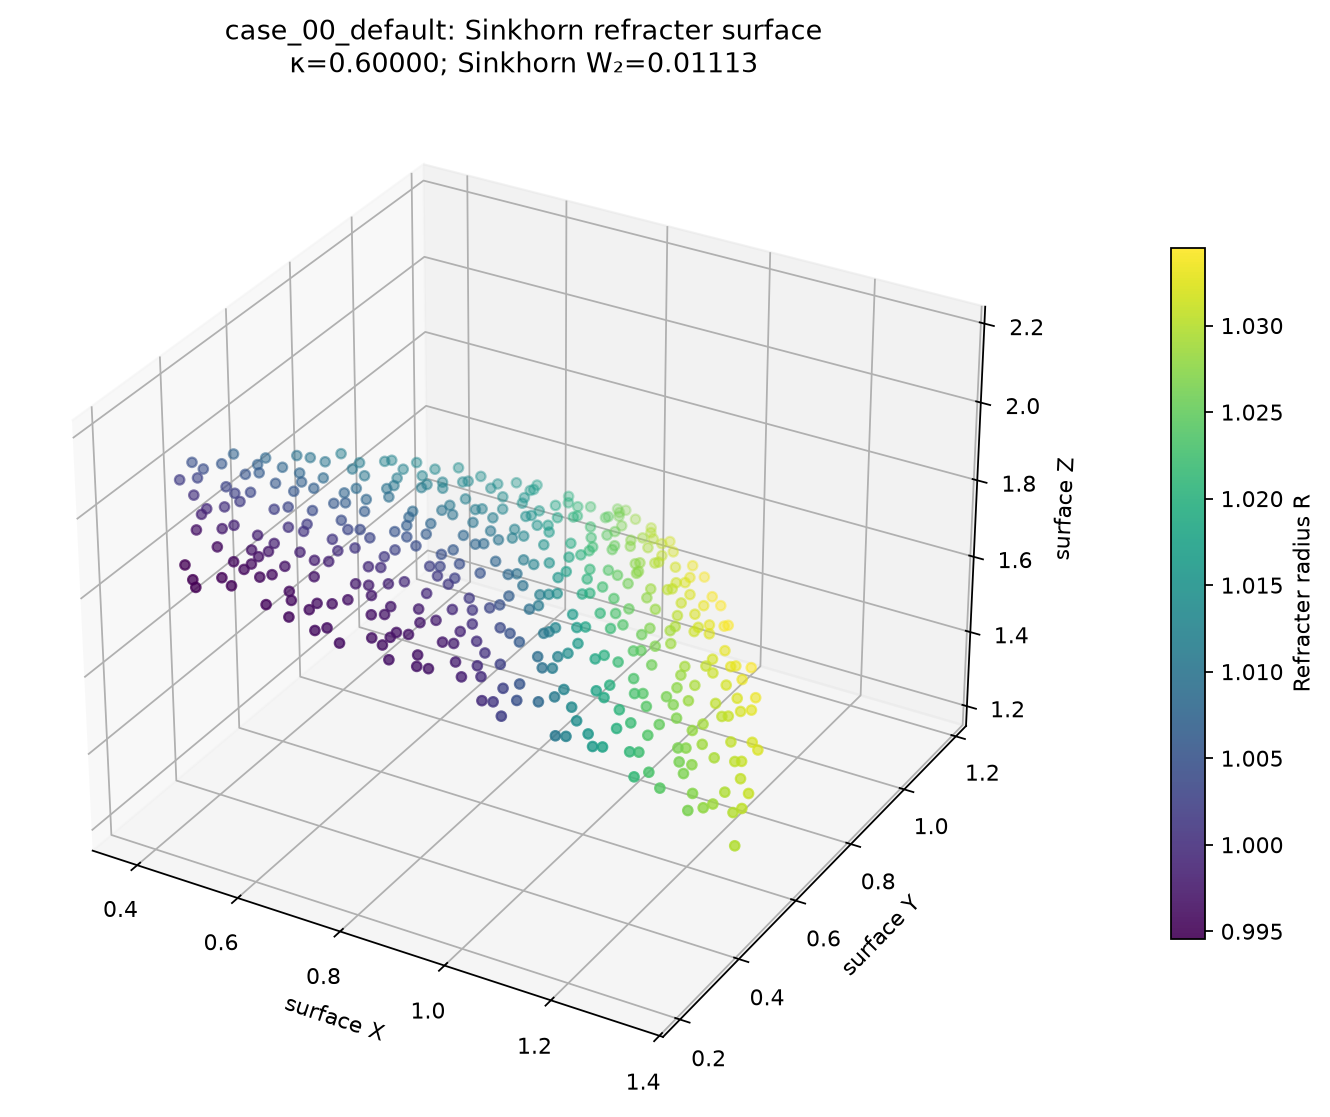
\includegraphics[width=0.48\textwidth]{case_00_default/case_00_default_surface_3d.png}\hfill
    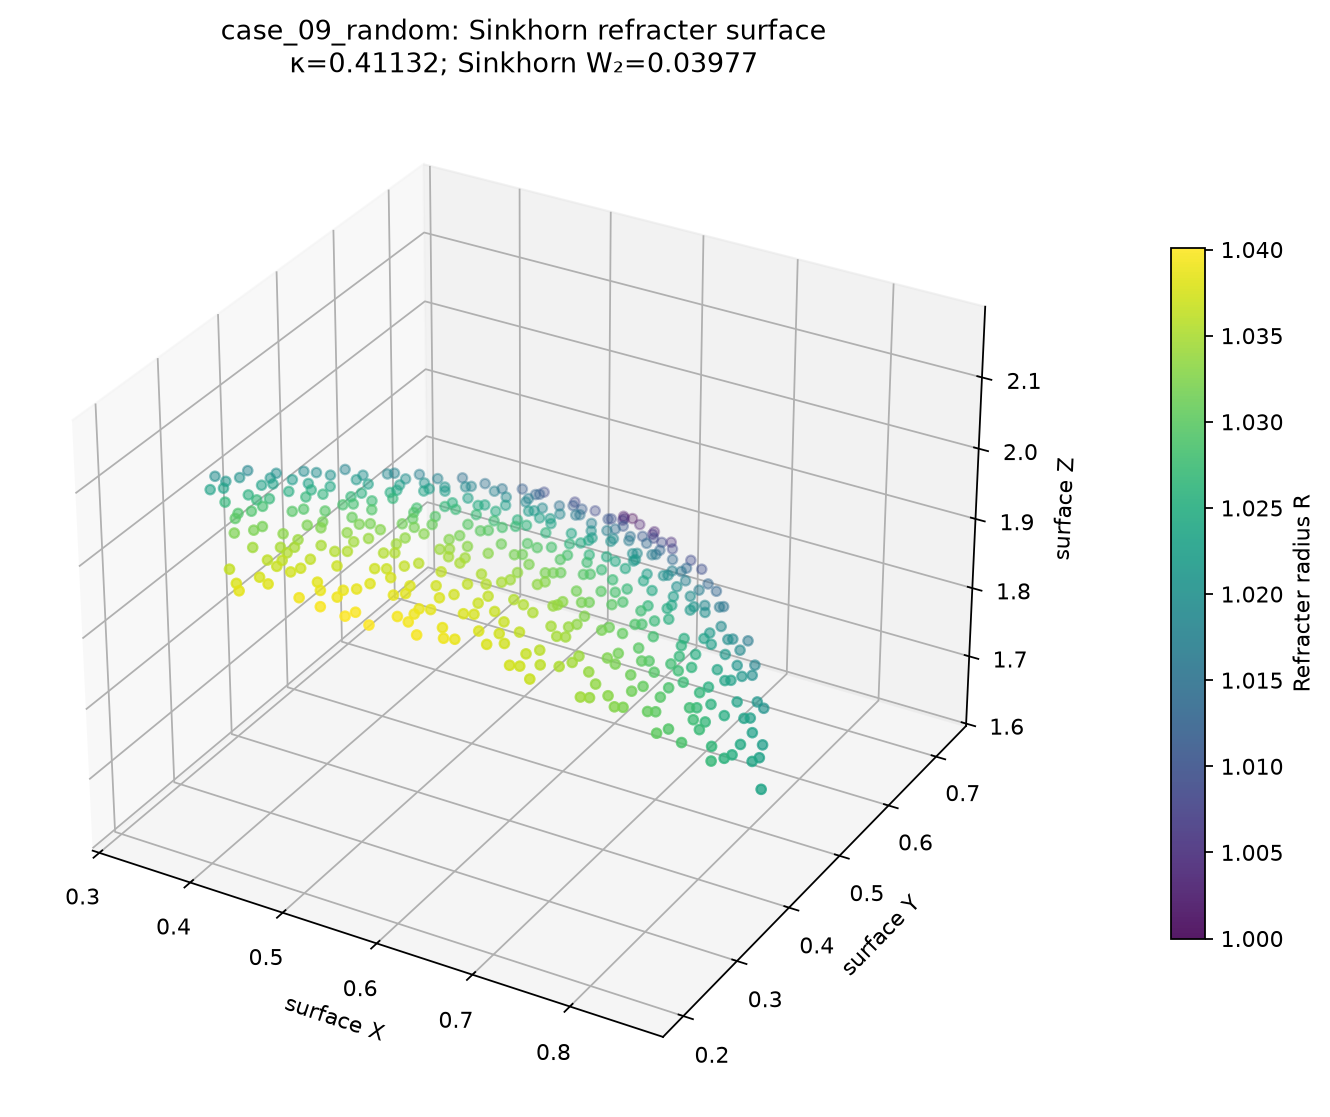
\includegraphics[width=0.48\textwidth]{case_09_random/case_09_random_surface_3d.png}
    \caption{Two representative refractor surfaces, coloured by $R$. Left:
    $\Omega_s=\{(1,\phi,\theta):\theta\in[\pi/12,\pi/3],\;
    \phi\in[\pi/12,\pi/4]\}$ and
    $\Omega_t=\{(1,\phi,\theta):\theta\in[\pi/10,\pi/5],\;
    \phi\in[\pi/10,\pi/5]\}$, with $\kappa=0.600000$ and
    $W_{\mathrm{radian}}=\text{to be updated}\,\mathrm{rad}$. Right:
    $\Omega_s=\{(1,\phi,\theta):\theta\in[0.3627,0.9582],\;
    \phi\in[0.2285,0.4861]\}$ and
    $\Omega_t=\{(1,\phi,\theta):\theta\in[0.8034,1.8359],\;
    \phi\in[0.4945,1.0514]\}$, with $\kappa=0.411324$ and
    $W_{\mathrm{radian}}=\text{to be updated}\,\mathrm{rad}$. All angular
    bounds are in radians; $\theta$ is azimuth and $\phi$ is polar angle.}
    \label{fig:week15-examples}
\end{figure}

\end{document}
